%!TEX root = ../PhDThesis.tex



% *********************************************************************************************************************
\chapter{Additional information about the first study}\label{app:studyinfo-pub}
% *********************************************************************************************************************



This appendix includes additional material to the first study of mobile device use in a pub (see \autoref{ch:empirical pub}):

\begin{itemize}
    \item \appref{app:studyinfo-pub infoconsent} provides the information sheet and consent form given to participants prior to the study,
    \item \appref{app:studyinfo-pub interview} provides the post-observation interview questions, and
%    \item \appref{app:studyinfo-pub questionnaire} provides the post-observation questionnaire
    \item \appref{app:studyinfo-pub datasession} provides the guidance on the study provided for the collaborative data session.
\end{itemize}

Additional material related to the study is available on the accompanying CD and online repository:

\begin{itemize}
    \item The descriptive results from the questionnaire are provided in \texttt{studyone/questionnaire.pdf}.
\end{itemize}



% *********************************************************************************************************************



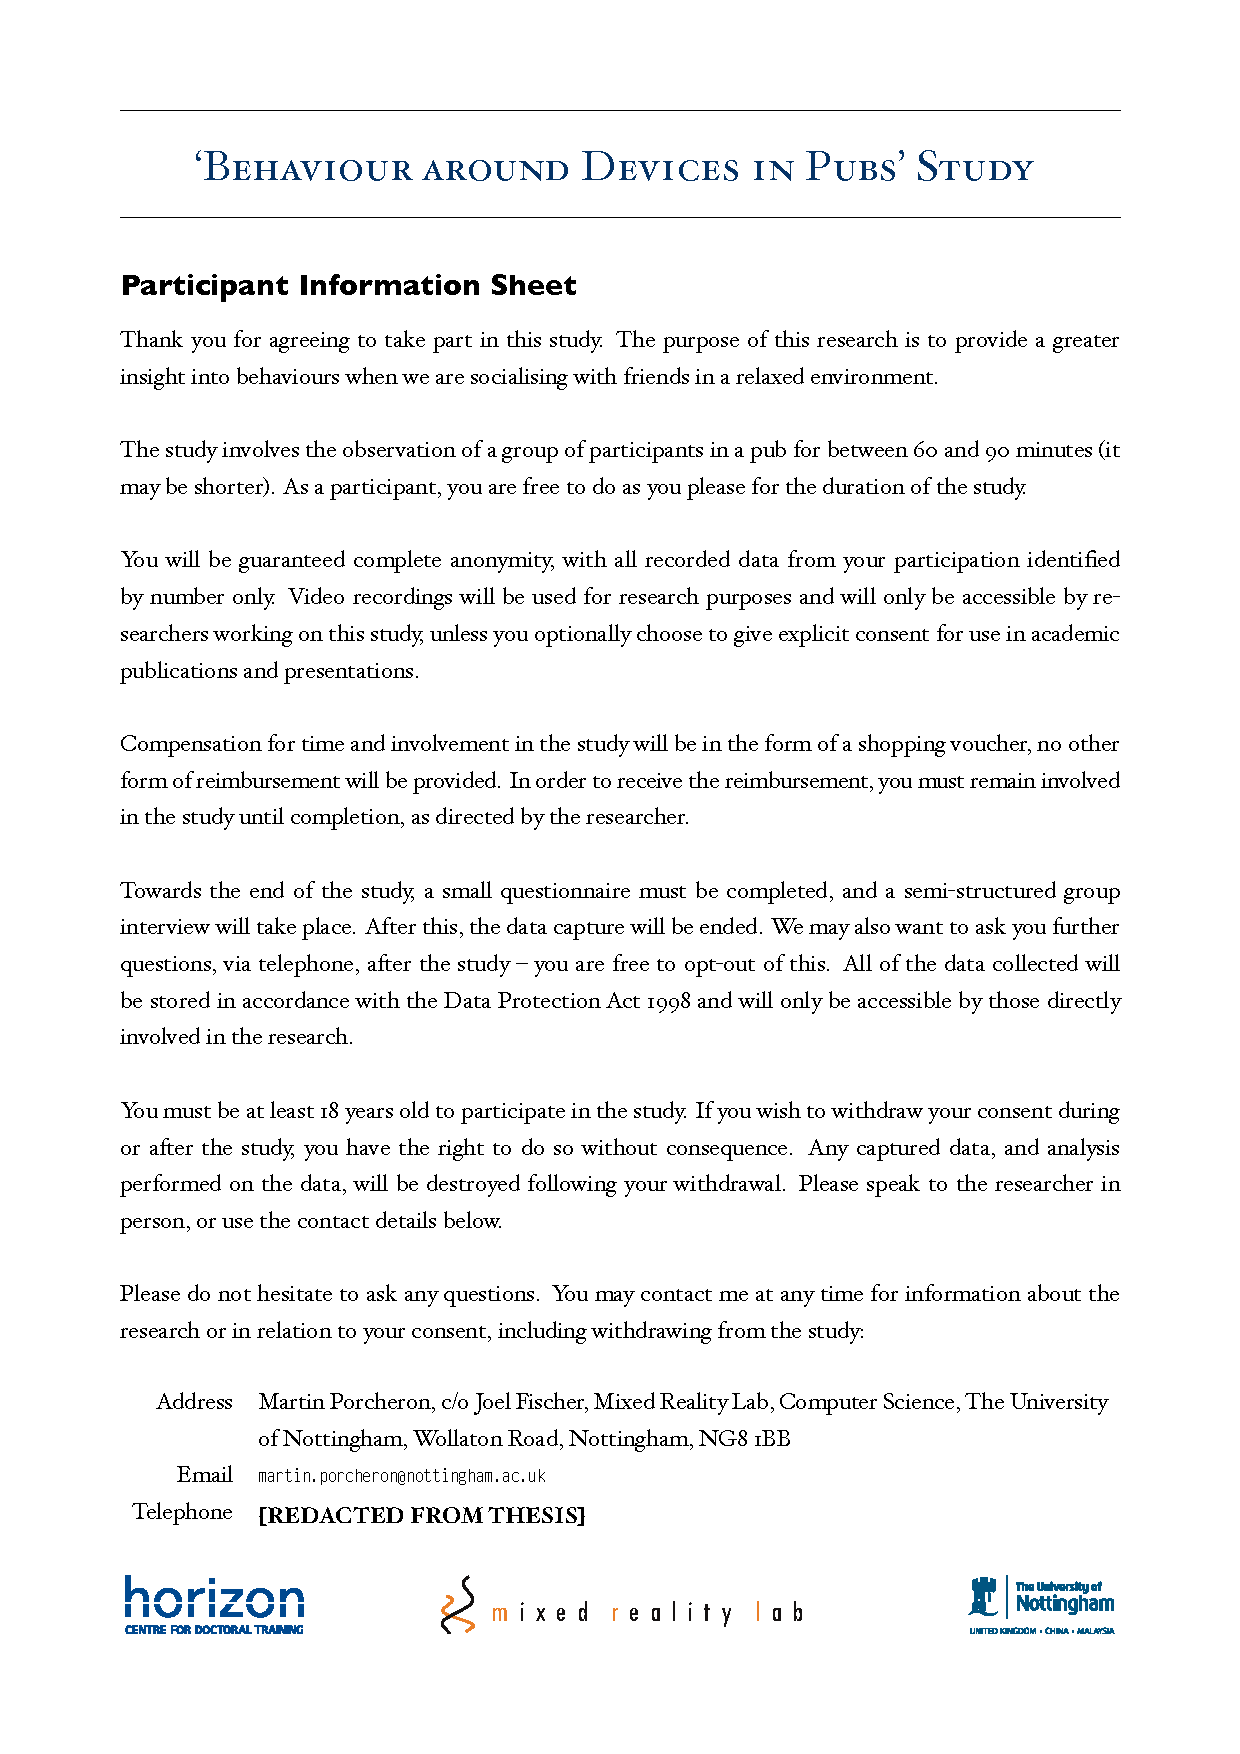
\includepdf[
    pages={1},
    scale=.6,
    frame=false,
    clip,
    trim=1.5cm 1.5cm 1.5cm 1.5cm,
    %offset=-1.05cm 0cm,
    pagecommand={\section{Information sheet and consent form}\label{app:studyinfo-pub infoconsent}}]
    {Graphics/A-StudyInfo-Pub/InfoConsent.pdf}
\includepdf[
    pages={2},
    scale=.6,
    frame=false,
    clip,
    trim=1.5cm 1.5cm 1.5cm 1.5cm,
    %offset=-1.05cm 0cm,
    pagecommand={\nopagebreak}]
    {Graphics/A-StudyInfo-Pub/InfoConsent.pdf}



% *********************************************************************************************************************



\section{Exit interview questions}\label{app:studyinfo-pub interview}

\begin{itemize}
    \item How do you feel about the presence of phones in social settings?
    \item Would you say the presence of devices has an impact on the conversation?
    \item Do you recall a time when you have felt ignored by someone using their phone?
    \item How feel about devices attempting to stop you using them at inopportune moments?
    \item Do you see any merits in devices attempting to restrict usage?
    \item Do you feel that people have a responsibility to the group dynamic?
    \item Would you categorise mobiles as a support tool or a distraction device
    \item Could you see mobile phones being used in conversation without detracting from it?
    \item Would you be willing to take part in further studies that required the installation of an app?
    \item Were you disturbed by presence of cameras or recording equipment?
    \item Did you feel you acted unnaturally due to nature of study?
    \item Did you remain aware of the presence of camera?
\end{itemize}



% *********************************************************************************************************************


% \includepdf[
%     pages={1},
%     scale=.6,
%     frame=false,
%     clip,
%     trim=1.5cm 1.5cm 1.5cm 1.5cm,
%     pagecommand={\section{Questionnaire}\label{app:studyinfo-pub questionnaire}}]
%     {Graphics/A-StudyInfo-Pub/Questionnaire.pdf}
% \includepdf[
%     pages={2},
%     scale=.6,
%     frame=false,
%     clip,
%     trim=1.5cm 1.5cm 1.5cm 1.5cm,
%     %offset=-1.05cm 0cm,
%     pagecommand={\nopagebreak}]
%     {Graphics/A-StudyInfo-Pub/Questionnaire.pdf}



% *********************************************************************************************************************



\section{Data session guidance}\label{app:studyinfo-pub datasession}



% *********************************************************************************************************************



\paragraph{Setting} \hfill \\
The recordings for this data session were made in a Nottingham-based pub, near to the university, during normal opening hours.
The majority of the recordings took place in the afternoon when the pub was relatively quiet.

A table that was in the corner of pub was chosen for the groups to sit at, and two GoPro cameras were positioned to capture all those present at the table.
One camera was positioned on a tripod and the other was positioned on a ledge within the pub.
An audio recorder was placed on the table to capture higher-quality audio.

Groups of 3 or 4 friends were recruited through email and word-of-mouth communication to participate in a study that involved “going to the pub”.
There were no prerequisites other than that all members of the group should be friends; groups were purposefully told minimal information before the study, other that what was required by the ethics committee.

Upon arrival at the pub, groups were greeted and invited to sort drinks out before taking their seats.
Consent forms were completed, and an opportunity for individuals to ask questions was provided.
The common question amongst groups was whether any tasks were required and this was answered accordingly.

The researcher sat at the table and engaged with the group where appropriate.



% *********************************************************************************************************************



\paragraph{Focus} \hfill \\
The focus of this research is to discover the interactional methods through which devices are topicalised, then sustained/co-oriented to, and then disengaged from, within social collocated interactions.



% *********************************************************************************************************************
